\section{Related Work}\label{sec:related}
\subsection{Domain-, Feature-, and Topology-Based Summaries}
Static views and animation distribute temporal comparison across space and time~\cite{Tversky:2002:Animation,Robertson:2008:Animation}; generalized space--time cubes describe transformations between these organizations~\cite{Bach:2017:STC}. Hovm\"oller diagrams retain a physical coordinate while aggregating the remaining dimensions~\cite{Hovmoller:1949}. Geographic orderings and space-filling curves traverse the spatial domain~\cite{Guo:2006:SpatialOrder,Dafner:2000:CSFC}, with extensions for volume comparison and scalar-aware traversal~\cite{Weissenboeck:2019:DVL,Zhou:2021:DSF}. Their coordinate records traversal rank, while averaging can merge nearby extrema.

Feature-based approaches organize selected entities and their motion, as in one-dimensional projections and MotionRugs~\cite{Franke:2021:1DP,Buchmueller:2019:MR}. Their emphasis differs from traversing every domain sample. Embeddings more generally balance original-domain relationships against display organization~\cite{Nonato:2019:MP}. Figure~\ref{fig:related-work-mapping} makes the distinction explicit: domain-based traversal retains samples, feature-based summaries select structures of interest, and topology-based profiles retain hierarchical relations. AnchorMTM builds on the last representation and assigns its extrema targets in a fixed physical projection.

\begin{figure}[!tb]
\centering
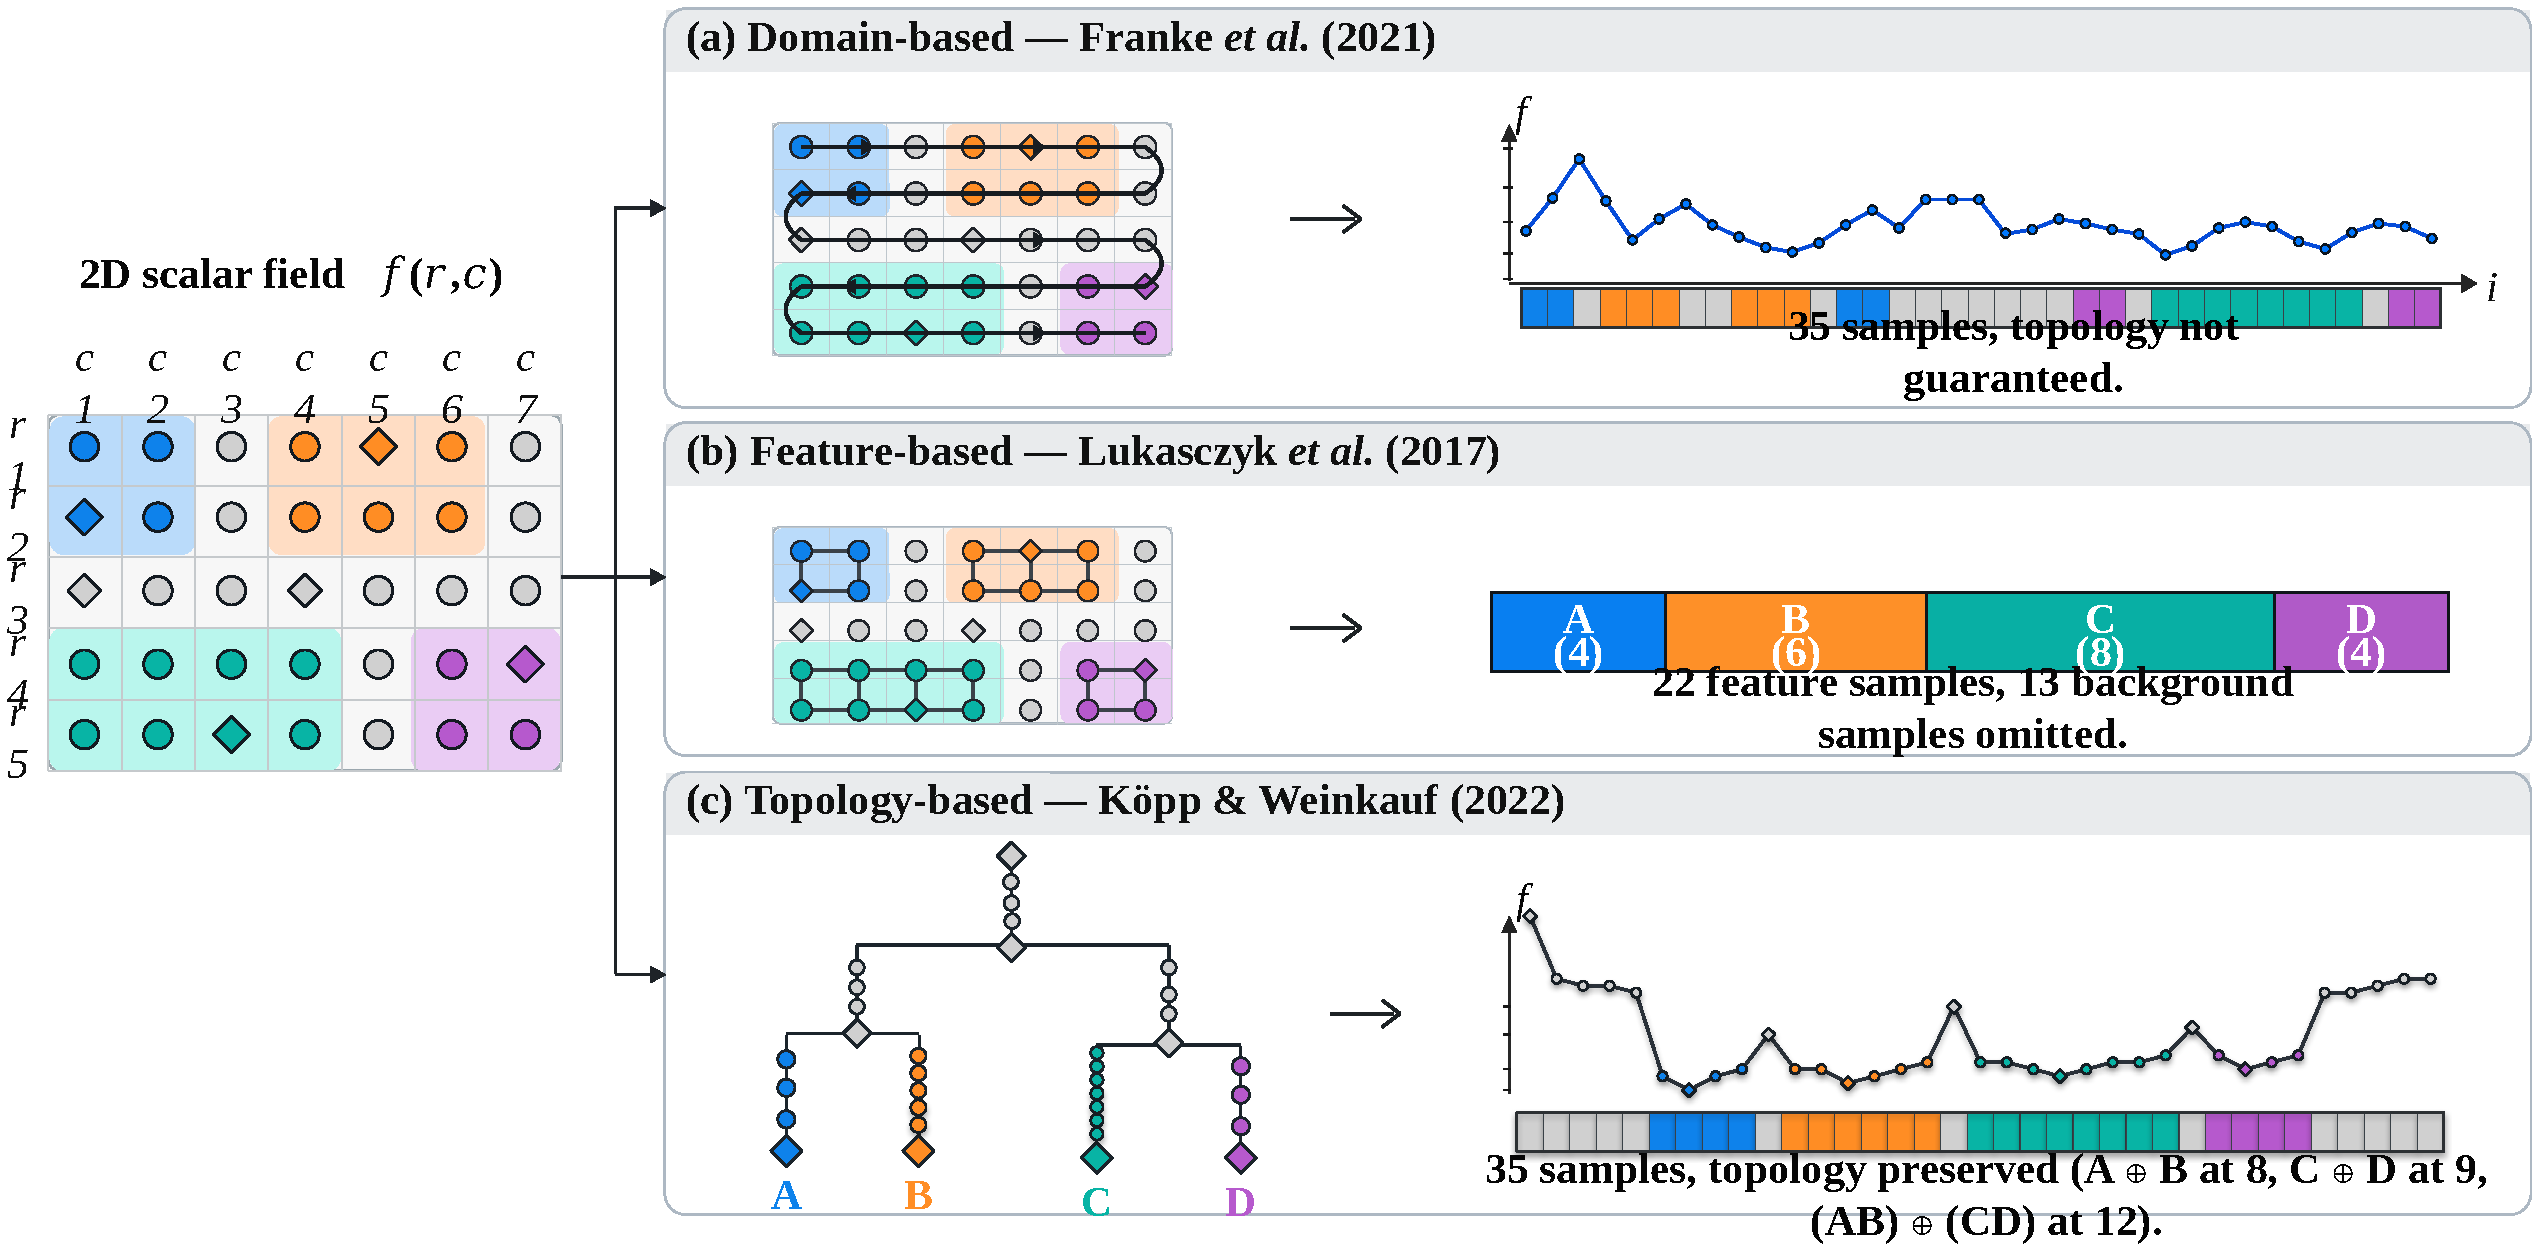
\includegraphics[width=\columnwidth]{figures/anchor_related_work_mapping.pdf}
\caption{Mapping strategies on a common 35-sample field: domain traversal; a 22-sample feature summary; and a topology-based profile retaining the complete illustrated hierarchy.}
\label{fig:related-work-mapping}
\end{figure}
\subsection{Topological Profiles and Constrained Layouts}
Topology-based representations organize scalar structures through connectivity~\cite{Heine:2016:Survey}. Landscapes and profiles turn the hierarchy into geometry~\cite{Weber:2007:TL,Oesterling:2013:TLP}, with extensions for spatial geometry and temporal coherence~\cite{Beketayev:2012:GPTL,Herick:2020:TCTL}. TMTM aligns these profiles through time~\cite{Koepp:2023:TMTM}; ST-MTM incorporates spatial-distance fitting and temporal constraints~\cite{STMTM:2026}. AnchorMTM retains that scalar-profile foundation. Its additional requirement is that one display coordinate refer to the same physical direction, origin and scale throughout the sequence.

Optimal leaf ordering minimizes adjacent dissimilarity subject to a hierarchy~\cite{BarJoseph:2001:OLO}; target-order reordering studies related compatible permutations~\cite{Bulteau:2022:RT}. Separation-constrained layouts manage overlap and displacement~\cite{Dwyer:2006:IPSEP,Li:2019:SOI}. Our bounds state the displacement that these ordering and packing constraints force relative to fixed targets. Merge-tree comparison depends on feature labels and correspondences~\cite{Yan:2021:Survey}; labelled cophenetic/interleaving representations support our fixed-identity merge-error measure~\cite{Munch:2019:LINF,Gasparovic:2024:IID}. Ordered merge trees connect scalar curves with interleaving distances~\cite{Beurskens:2025:OMT}, and minimax ultrametric fitting provides a related setting for correcting merge levels~\cite{Farach:1995:RM}.
